\documentclass[12pt,a4paper]{article}
\usepackage[margin=1in]{geometry}
\usepackage{listings}
\usepackage{xcolor}
\usepackage{hyperref}
\usepackage{enumitem}
\usepackage{tikz}
\usetikzlibrary{arrows.meta, positioning}

\definecolor{codebg}{RGB}{245,242,234}
\definecolor{codetext}{RGB}{28,37,65}
\definecolor{keyword}{RGB}{161,101,47}
\definecolor{comment}{RGB}{114,108,94}

\lstset{
  backgroundcolor=\color{codebg},
  basicstyle=\ttfamily\small\color{codetext},
  keywordstyle=\color{keyword}\bfseries,
  commentstyle=\color{comment}\itshape,
  breaklines=true,
  frame=single,
  rulecolor=\color{comment},
  xleftmargin=6pt,
  xrightmargin=6pt,
  aboveskip=10pt,
  belowskip=10pt
}

\title{\textbf{IIT Ropar Classroom Booking System} \\ \large AI511 Lab 6 -- Code Walkthrough}
\author{Dhakshin K \\ 2024AIB1009}
\date{September 2026}

\begin{document}
\maketitle
\tableofcontents
\newpage

% ---------------------------------------------------------------
\section{Project Overview}

A browser-based prototype for booking classrooms at IIT Ropar. No backend, no framework -- just HTML, CSS, and vanilla JavaScript. All data is stored in the browser's \texttt{localStorage}.

Three user roles:
\begin{itemize}
  \item \textbf{Student} -- books rooms, views status
  \item \textbf{Admin} -- approves, rejects, suggests alternatives
  \item \textbf{Security} -- checks in/out, records room condition
\end{itemize}

% ---------------------------------------------------------------
\section{File Structure}

\begin{lstlisting}
classroom-booking/
  index.html        <- page structure (all screens)
  README.md         <- documentation
  css/
    style.css       <- all visual styling
  js/
    data.js         <- demo users, rooms, timetable
    booking.js      <- availability check, booking creation
    admin.js        <- approve / reject / suggest alternative
    security.js     <- QR check-in, check-out
    app.js          <- navigation, rendering, localStorage
\end{lstlisting}

% ---------------------------------------------------------------
\section{What Each File Does}

\subsection{index.html -- Page Structure}

Contains all the screens as \texttt{<section>} tags. Only one section is visible at a time (controlled by the \texttt{show()} function in \texttt{app.js}). The screens are:

\begin{enumerate}
  \item \textbf{Login} -- email + password form
  \item \textbf{Home} -- landing page with live room board
  \item \textbf{Student Dashboard} -- stats, timetable, my bookings
  \item \textbf{Calendar} -- full weekly timetable view
  \item \textbf{Book a Room} -- form with room picker
  \item \textbf{Confirmation} -- shown after booking is submitted
  \item \textbf{Admin Dashboard} -- pending requests + all bookings
  \item \textbf{Security} -- QR scan, occupied rooms, check-out
  \item \textbf{Notifications} -- per-user notification feed
\end{enumerate}

No logic lives here. Just layout and references to CSS/JS files.

\subsection{css/style.css -- Styling}

All visual design in one file. Uses CSS custom properties (design tokens):

\begin{lstlisting}[language=CSS]
:root {
  --ink: #1c2541;       /* main text */
  --brass: #a1652f;     /* accent / buttons */
  --teal: #1f6f5c;      /* success / available */
  --rust: #a13d3d;      /* error / occupied */
  --paper: #f5f2ea;     /* background */
}
\end{lstlisting}

Key CSS classes: \texttt{.card}, \texttt{.badge}, \texttt{.btn}, \texttt{.room-option}, \texttt{.toast}.

Responsive -- uses media queries for mobile layout.

\subsection{js/data.js -- Demo Data}

Three constant arrays:

\begin{itemize}
  \item \textbf{\texttt{demoUsers}} -- 3 accounts with email, password, role, name
  \item \textbf{\texttt{rooms}} -- 6 campus rooms with code and capacity
  \item \textbf{\texttt{timetable}} -- 8 academic course entries with room, days, start/end times
\end{itemize}

The timetable is the \textbf{hard constraint} -- rooms cannot be booked during scheduled classes.

Example timetable entry:
\begin{lstlisting}[language=Java]
{ course: "CS111",
  title: "Intro to Programming",
  room: "CS-1",
  days: ["Tuesday", "Thursday"],
  start: "15:00",
  end: "16:00" }
\end{lstlisting}

\subsection{js/booking.js -- Availability and Booking Creation}

This is the \textbf{most important file} for the core problem (classroom clashes).

\subsubsection{isRoomAvailable(roomCode, date, startTime, endTime)}

The central function. Checks two things:

\begin{enumerate}
  \item \textbf{Academic timetable} -- loops through \texttt{timetable[]}. If the room is scheduled for a class on that day and the times overlap, returns \texttt{\{available: false, reason: "..."\}}.
  \item \textbf{Existing bookings} -- loops through all bookings in localStorage. If any Pending/Approved/Occupied booking for the same room and date overlaps in time, returns unavailable.
\end{enumerate}

\begin{lstlisting}[language=Java]
function isRoomAvailable(roomCode, date, startTime, endTime) {
  // 1. check timetable conflicts
  for (const entry of timetable) {
    if (entry.room === roomCode
        && entry.days.includes(getDayName(date))) {
      if (timesOverlap(startTime, endTime,
                        entry.start, entry.end)) {
        return { available: false,
                 reason: "Academic class ..." };
      }
    }
  }
  // 2. check existing bookings
  for (const b of getBookings()) {
    if (b.room === roomCode && b.date === date
        && ["Approved","Occupied","Pending"]
            .includes(b.status)) {
      if (timesOverlap(startTime, endTime,
                        b.startTime, b.endTime)) {
        return { available: false,
                 reason: "Existing booking ..." };
      }
    }
  }
  return { available: true };
}
\end{lstlisting}

\subsubsection{timesOverlap(s1, e1, s2, e2)}

Simple overlap check. Two time ranges overlap if one starts before the other ends:

\begin{lstlisting}[language=Java]
function timesOverlap(s1, e1, s2, e2) {
  return s1 < e2 && s2 < e1;
}
\end{lstlisting}

Times are strings like \texttt{"15:00"} -- string comparison works because they're zero-padded.

\subsubsection{getAvailableRooms(date, startTime, endTime, attendees)}

Calls \texttt{isRoomAvailable()} for every room in the \texttt{rooms[]} array. Also checks if \texttt{room.capacity >= attendees}. Returns an array of rooms with availability info, which powers the room picker UI.

\subsubsection{validateAndCreateBooking(...)}

Takes all form inputs (purpose, attendees, date, start, end, room, notes). Does three things:
\begin{enumerate}
  \item Validates required fields (missing purpose? no date? no room selected?)
  \item Final availability check at submit time
  \item Creates the booking object with status \texttt{"Pending"} and saves to localStorage
\end{enumerate}

The booking object:
\begin{lstlisting}[language=Java]
{
  id: "IITRPR-48291",
  student: "student@iitrpr.ac.in",
  room: "CS-1",
  date: "2026-09-25",
  startTime: "15:00",
  endTime: "17:00",
  purpose: "Coding Club Workshop",
  attendees: 70,
  status: "Pending",
  qrToken: null   // set when approved
}
\end{lstlisting}

\subsection{js/admin.js -- Admin Actions}

Three functions that change booking state:

\subsubsection{approveBooking(bookingId)}
\begin{itemize}
  \item Sets \texttt{status = "Approved"}
  \item Generates QR token: \texttt{qrToken = "QR-IITRPR-48291"}
  \item Sends notification to the student
\end{itemize}

\subsubsection{rejectBooking(bookingId, remark)}
\begin{itemize}
  \item Sets \texttt{status = "Rejected"}
  \item Stores the admin's reason in \texttt{adminRemark}
  \item Sends notification to the student
\end{itemize}

\subsubsection{suggestAlternative(bookingId, altRoom)}
\begin{itemize}
  \item First checks if the alternative room is actually available (calls \texttt{isRoomAvailable})
  \item Sets \texttt{status = "Alternative Suggested"}
  \item Stores \texttt{alternativeRoom = "CS-1"}
  \item Student then sees Accept/Decline buttons
\end{itemize}

\texttt{acceptAlternative()} swaps the room and sets status to Approved. \texttt{declineAlternative()} sets status to Rejected.

\subsection{js/security.js -- Check-in and Check-out}

\subsubsection{checkInBooking(qrToken)}
\begin{itemize}
  \item Finds booking by QR token
  \item Verifies status is \texttt{"Approved"} (can't check in a pending booking)
  \item Sets \texttt{status = "Occupied"}, records \texttt{checkinTime}
\end{itemize}

\subsubsection{checkOutBooking(bookingId, conditionRemark)}
\begin{itemize}
  \item Verifies status is \texttt{"Occupied"}
  \item Sets \texttt{status = "Completed"}, records \texttt{checkoutTime}
  \item Stores condition remark (e.g. ``No damage observed'', ``Projector issue'')
  \item Notifies student and admin
\end{itemize}

\subsection{js/app.js -- Navigation, State, Rendering}

The largest file. Connects everything together.

\subsubsection{Key state}
\begin{lstlisting}[language=Java]
var currentUser = null;   // set on login
var selectedRoom = null;  // set in room picker
\end{lstlisting}

\subsubsection{localStorage helpers}
\begin{lstlisting}[language=Java]
getBookings()      // read bookings from localStorage
saveBookings(arr)  // write bookings to localStorage
addNotification(recipient, text, type)
\end{lstlisting}

All data persists across page refresh.

\subsubsection{show(id) -- Navigation}

Hides all \texttt{<section>} elements, shows the requested one. Also refreshes the content (calls the right render function) and updates the active nav tab.

\subsubsection{handleLogin()}

Matches email + password against \texttt{demoUsers[]}. Sets \texttt{currentUser} with role, name, email. Calls \texttt{updateNav()} which builds role-specific navigation tabs:
\begin{itemize}
  \item Student sees: Home, Dashboard, Book a Room, Notifications
  \item Admin sees: Home, Admin Dashboard, Notifications
  \item Security sees: Home, Security, Notifications
\end{itemize}

\subsubsection{updateRoomPicker()}

Called automatically when date/time inputs change (via event listeners). Calls \texttt{getAvailableRooms()} and renders room buttons -- available rooms are clickable, unavailable rooms are disabled with the conflict reason shown.

\subsubsection{Rendering functions}

Each page has a render function:
\begin{itemize}
  \item \texttt{renderStudentDashboard()} -- stats cards, today's timetable, booking list with status badges
  \item \texttt{renderAdminDashboard()} -- pending request table with Approve/Reject/Suggest buttons
  \item \texttt{renderSecurityPage()} -- QR scan area, occupied rooms list with checkout buttons
  \item \texttt{renderNotifications()} -- filtered by current user's email
  \item \texttt{renderBoard()} -- home page room board with live status
\end{itemize}

% ---------------------------------------------------------------
\section{Booking Lifecycle}

This is the core state machine of the application:

\begin{center}
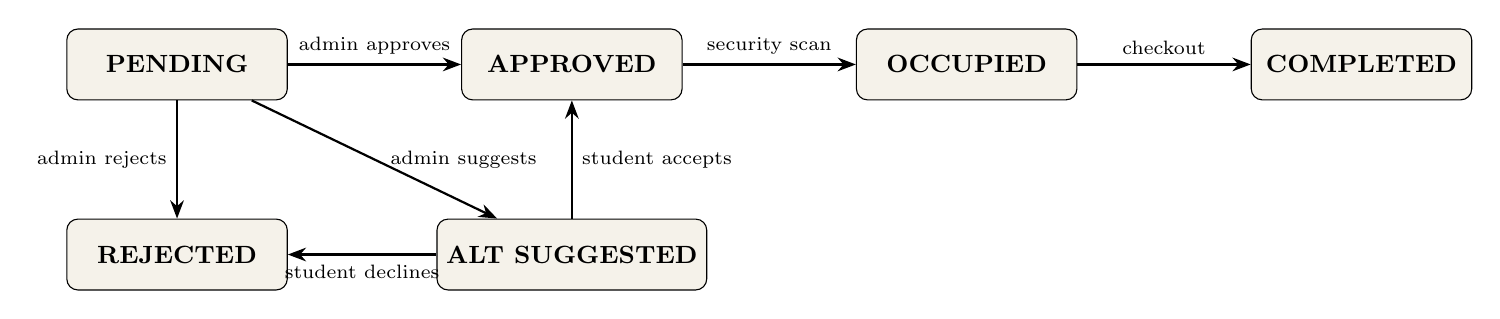
\begin{tikzpicture}[
  node distance=2.2cm,
  state/.style={rectangle, draw, rounded corners, fill=codebg, minimum width=2.8cm, minimum height=0.9cm, font=\small\bfseries},
  every edge/.style={draw, -Stealth, thick}
]
  \node[state] (pending)   {PENDING};
  \node[state, right=of pending] (approved) {APPROVED};
  \node[state, right=of approved] (occupied) {OCCUPIED};
  \node[state, right=of occupied] (completed) {COMPLETED};

  \node[state, below=1.5cm of pending] (rejected) {REJECTED};
  \node[state, below=1.5cm of approved] (alt) {ALT SUGGESTED};

  \path (pending)  edge node[above, font=\scriptsize] {admin approves} (approved);
  \path (approved) edge node[above, font=\scriptsize] {security scan} (occupied);
  \path (occupied) edge node[above, font=\scriptsize] {checkout} (completed);

  \path (pending) edge node[left, font=\scriptsize] {admin rejects} (rejected);
  \path (pending) edge node[right, font=\scriptsize, xshift=2pt] {admin suggests} (alt);
  \path (alt) edge node[right, font=\scriptsize] {student accepts} (approved);
  \path (alt) edge node[below, font=\scriptsize] {student declines} (rejected);
\end{tikzpicture}
\end{center}

Each arrow is a \textbf{function call} that modifies the booking object in localStorage and triggers a notification.

% ---------------------------------------------------------------
\section{Conflict Detection -- How It Works}

When a student selects a date and time in the booking form:

\begin{enumerate}
  \item Event listeners on the date/time inputs call \texttt{updateRoomPicker()}
  \item \texttt{updateRoomPicker()} calls \texttt{getAvailableRooms(date, start, end, attendees)}
  \item For each of the 6 rooms, \texttt{isRoomAvailable()} runs:
    \begin{itemize}
      \item Loop through \texttt{timetable[]} -- check if any class uses that room on that day with overlapping time
      \item Loop through \texttt{getBookings()} -- check if any active booking uses that room on that date with overlapping time
    \end{itemize}
  \item The room picker renders: available rooms are green/clickable, blocked rooms are greyed out with the conflict reason (e.g. ``CS111 scheduled 3:00--4:00 PM'')
\end{enumerate}

Example conflict:
\begin{lstlisting}
Request:  CS-1, Tuesday, 2:30 PM - 4:30 PM
Timetable: CS-1, Tuesday, 3:00 PM - 4:00 PM (CS111)

timesOverlap("14:30", "16:30", "15:00", "16:00")
  -> "14:30" < "16:00" && "15:00" < "16:30"
  -> true && true
  -> CONFLICT

Result: CS-1 shows as disabled, reason displayed
\end{lstlisting}

% ---------------------------------------------------------------
\section{localStorage Persistence}

Three keys stored in the browser:

\begin{center}
\begin{tabular}{|l|l|}
\hline
\textbf{Key} & \textbf{What it stores} \\
\hline
\texttt{currentUser} & logged-in user (email, role, name) \\
\texttt{bookings} & array of all booking objects \\
\texttt{notifications} & array of notification objects \\
\hline
\end{tabular}
\end{center}

On page load, \texttt{app.js} checks if \texttt{currentUser} exists in localStorage. If yes, it restores the session and navigates to the right dashboard. This means refreshing the page doesn't lose your data.

% ---------------------------------------------------------------
\section{Demo Flow for Presentation}

Follow this exact sequence to show the full lifecycle:

\begin{enumerate}
  \item Login as \texttt{student@iitrpr.ac.in}
  \item Go to ``Book a Room'' -- pick a date, set time to 3:00--5:00 PM
  \item Watch the room picker update -- some rooms will show as unavailable
  \item Select an available room, type a purpose, submit
  \item See the booking as \textbf{PENDING} in the dashboard
  \item Logout, login as \texttt{admin@iitrpr.ac.in}
  \item See the pending request -- click \textbf{Approve}
  \item Logout, login as \texttt{student@iitrpr.ac.in}
  \item See status changed to \textbf{APPROVED}, click ``View QR Code''
  \item Logout, login as \texttt{security@iitrpr.ac.in}
  \item Select the QR token from dropdown, click ``Simulate scan''
  \item Room shows as \textbf{OCCUPIED}
  \item Select a condition remark, click ``Check Out''
  \item Room is now \textbf{COMPLETED} / available
\end{enumerate}

This single flow covers: booking creation, validation, conflict detection, admin approval, QR generation, check-in, check-out, and room condition -- all the marking criteria.

\end{document}
